%! TeX program = pdflatex
%! TeX options = -synctex=1 -interaction=nonstopmode -halt-on-error
% IEEE Access submission root.  The manuscript prose remains modular under
% ../a_abstract through ../g_conclusion; do not move section content here.
\documentclass{ieeeaccess}

% Packages used by the modular manuscript.
\usepackage{amsmath,amssymb,amsfonts}
\usepackage{booktabs}
\usepackage{array}
\usepackage{tabularx}
\usepackage{longtable}
\usepackage{graphicx}
\usepackage{float}
\usepackage{xurl}
\usepackage[hidelinks]{hyperref}
\usepackage[numbers,sort&compress]{natbib}

% Paths are relative to this IEEE Access template folder.
\graphicspath{{../e_result/figures/}{../figures/}{../images/}}
\makeatletter
\def\input@path{{../}}
\makeatother

\begin{document}

% Leave publication history and DOI unset: IEEE supplies these after acceptance.
\history{}
\doi{}
\title{Epoch-Aware Threshold Estimation for Blink Detection in Naturalistic Driving EEG
}

% Rodney Petrus Balandong is first and corresponding author.
\author{\uppercase{Rodney Petrus Balandong}\authorrefmark{1,2},
\uppercase{Nur Syahirah Roslan}\authorrefmark{3},
\uppercase{Syaimaa' Solehah Mohd Radzi}\authorrefmark{2},
\uppercase{Muhamad Hafiz Abd Latif}\authorrefmark{2}, and
\uppercase{Tong Boon Tang}\authorrefmark{2}}

\address[1]{Green Technologies and Advanced Matter (GreAt) Research Group,
Faculty of Science and Natural Resources, Universiti Malaysia Sabah,
88400 Kota Kinabalu, Sabah, Malaysia}
\address[2]{Centre for Intelligent Signal and Imaging Research (CISIR),
Universiti Teknologi PETRONAS, 32610 Seri Iskandar, Perak, Malaysia}
\address[3]{Department of Information Systems, Faculty of Information and
Communication Technology, Universiti Tunku Abdul Rahman, Perak, Malaysia}

\tfootnote{This research was supported by the Ministry of Higher Education (MOHE) under the Fundamental Research Grant Scheme -- Early Career Researcher (FRGS-EC) with the project code (FRGC026-2024).}

\markboth
{Balandong \headeretal: Epoch-Aware Threshold Estimation for Blink Detection}
{Balandong \headeretal: Epoch-Aware Threshold Estimation for Blink Detection}

\corresp{Corresponding author: Rodney Petrus Balandong (e-mail: balandong@ums.edu.my).}

\begin{abstract}
In fatigue-driving studies, blink activity within the electroencephalography (EEG) is treated as marker of driver fatigue rather than noise. Thresholding is one of the most straightforward and widely used approaches for detecting blink activity from EEG signals. However, current approaches that use thresholding estimate a single amplitude threshold from a pool of blink-heavy and blink-free epochs concatenated together, which dilutes the amplitude statistics used for threshold estimation. This study presents an epoch-aware, three-stage pipeline that avoids this dilution by keeping blink-heavy and blink-free epochs separate when estimating the detection threshold. The three-stage pipeline first screened non-overlapping epochs by peak-to-peak amplitude, then estimated a sample-level threshold from the suspicious-epoch pool, and finally extracted blink regions and mapped them to epoch-local coordinates. The proposed pipeline and two established continuous-signal baselines were compared on the complete 32-channel montage using two naturalistic driving-EEG corpora, an internally collected dataset and  public dataset, evaluated with event-level overlap matching and macro-averaged $F_1$. Evaluated on this 32-channel montage configuration, the proposed pipeline reached macro-$F_1$ scores of 88.25\% on Internal and 80.68\% on public dataset, significantly exceeding both baselines on both corpora after Bonferroni-corrected Wilcoxon signed-rank tests. These results indicate that epoch-aware threshold estimation yields more reliable blink detection than continuous-signal thresholding in naturalistic EEG driving recordings.
\end{abstract}


\begin{keywords}
blink detection, electroencephalography, epoch-aware detection, naturalistic
driving, threshold selection
\end{keywords}

\titlepgskip=-15pt
\maketitle

% The introduction follows a paragraph-per-file structure (one paragraph, one
% file) as required by instruction_agentic/rule/latex_writing_rule.md.
\section{Introduction}

\input{b_intro/p001/paragraph}

\input{b_intro/p002/paragraph}

%\input{b_intro/p003/paragraph}

%\input{b_intro/p004/paragraph}
\input{b_intro/p004/paragraph_compress}

\input{b_intro/p005/paragraph}

%\input{b_intro/p006/paragraph}

\input{b_intro/p007/paragraph}
\input{b_intro/p008/paragraph}
%
\section{Related Work}
%file:///C:/Users/balan/Downloads/peerj-cs-3249.pdf

%However, most of these methods require empirically preset  conditions, and few have explored whether the boundaries of blink artifact intervals are  accurately recognized. Amplitude thresholding, which is based on a priori estimation of  blink artifact amplitude, achieves the detection of blink peaks and thus blink position  localization

% add also study by https://www.sciencedirect.com/science/article/pii/S0165027010003894?via%3Dihub:Currently, the primary methods to detect blink artifacts involve amplitude thresholding
%(Nolan, Whelan & Reilly, 2010),
The classical literature established the difficulty of ocular contamination and motivated automated statistical detection directly from EEG. Early work emphasized artifact removal and statistical screening rather than blink-region benchmarking per se, but it already showed that extreme-value behavior, channel context, and morphology matter \citep{croft2000removal,klein2013reliable}. This historical backdrop explains why simple one-value global thresholds can be attractive, yet brittle.

A first important stream comprises single-channel or few-channel threshold-centered detectors. Chang et al.~\citep{chang2016detection} detect blink artifacts from a single prefrontal channel using digital filtering and rule-based decisions. Tran et al.~\citep{tran2021detection} present an explicitly thresholding-based EEG blink detector and compute a minimum amplitude threshold from transformed signal magnitude and signal standard deviation. Zhang et al.~\citep{zhang2023method} move toward real-time frontal EEG detection with short windows and decision logic around potential blink boundaries. Wang et al.~\citep{wang2022multidimensional} extend thresholding to harder clinical settings by optimizing multidimensional features in the presence of epileptiform discharges, and later work based on higher-order cumulants continues the move toward short-segment single-channel detection \citep{wang2025sliding}.

A second stream contains hybrid thresholding pipelines. BLINKER first identifies candidate intervals with a mean-based standard-deviation threshold and then rejects implausible candidates using robust amplitude-distribution criteria derived from the median absolute deviation \citep{kleifges2017blinker}. Cao et al.~\citep{cao2021unsupervised} use cascaded thresholding over amplitude, amplitude displacement, and cross-channel correlation before applying a Gaussian mixture model. Agarwal et al.~\citep{agarwal2019blink} self-learn user-specific profiles in an unsupervised manner, while Valderrama et al.~\citep{valderrama2018automatic} use iterative template matching and automatic threshold/template estimation for suppression in single-channel recordings. Guttmann et al.~\citep{guttmann2019new} further emphasize adaptation to inter- and intra-subject variability, underscoring that fixed thresholds are often not enough.





%Therefore, it is necessary to establish an assumption-free detection approach capable of  adaptively and more precisely identifying blink artifacts of varying durations by exploiting  the inherent characteristic distinctions between EEG signals and blink artifacts.

%A growing stream of blink and ocular-artifact research replaces hand-tuned thresholds with data-driven models. Convolutional neural networks have been used both to detect eye-blink artifacts and to remove them from EEG~\citep{jurczak2022implementation,gawande2022deep}, while transformer- and video-based architectures have pushed blink-detection accuracy further~\citep{fodor2023blinklinmult,hong2024robust}. Autoencoder and segmentation-denoising networks also target single-channel artifact removal~\citep{faisal2025eye,li2023segmentation}, and recent reviews catalogue the broader shift from conventional thresholding toward deep learning for physiological-artifact handling, including in wearable EEG~\citep{akshathraj2026physiological,arpaia2025systematic}. In driving and fatigue monitoring, machine-learning and CNN models detect drowsiness from blink and eye-state cues~\citep{cabot2024drowsiness,makhmudov2024real}. These data-driven detectors can be accurate, but they typically require labelled training data, more computation, and offer less transparency than a single interpretable threshold. This contrast motivates studying the lightweight thresholding stage itself, which frequently precedes or complements such pipelines, and in particular the epoch-structure estimation bias that this paper addresses.

\section{METHOD AND MATERIALS}\label{sec:method}
%\input{d_method/m_pipeline_overview}
%
%
%\input{d_method/step1_select_bad_epoch}
%\input{d_method/step2_get_threshold_candidates}
%\input{d_method/step3_get_blink_regions}

\input{d_method/experiment_setup}
\section{Results}
\label{sec:results}



% =====================================================================
% EXPERIMENT 1 — channel selection
% =====================================================================
\subsection{Experiment 1: EEG Channel-Subset Analysis}
\label{sec:exp1_channel}
\input{e_result/exp1/sec}


% =====================================================================
% EXPERIMENT 2 — epoch duration
% =====================================================================
\subsection{Experiment 2: Stability Across Epoch Durations}
\label{sec:exp3_epoch}

\input{e_result/exp2/sec}



% NOTE (commented out on purpose, do not delete): this ablation ("Effect of the Threshold
% Estimator at Stage B") was archived to e_result/obs/exp3/sec.tex since it is not part of
% the active flow. Re-enable by moving that folder back and uncommenting here; see
% e_result/obs/README.md.
% \subsection{Effect of the Threshold Estimator at Stage B}
% \label{sec:estimator}
% \input{e_result/obs/exp3/sec}




% =====================================================================
% EXPERIMENT 3 — strategy comparison
% =====================================================================
\subsection{Experiment 3: Strategy Comparison}
\label{sec:exp3_strategy}
\input{e_result/exp3/sec}

%\subsection{Operating Points}
%\label{sec:operating_points}

%\begin{figure}[ht]
%    \centering
%    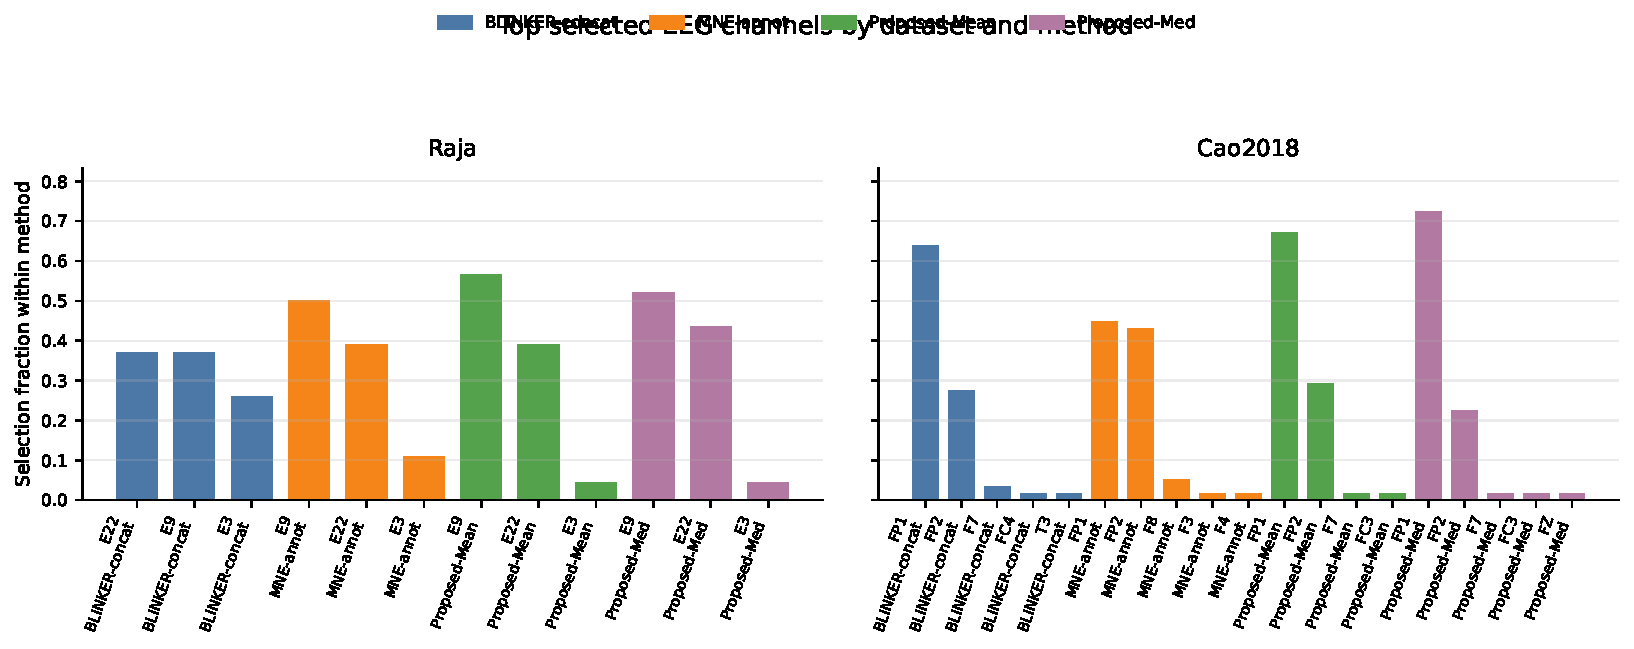
\includegraphics[width=0.9\linewidth]{fig_channel_selection.pdf}
%    \caption{Best-channel selection frequency, pooled over the four conditions.}
%    \label{fig:channel_selection}
%\end{figure}


\section{Discussion}
\label{sec:discussion}

\input{f_discussion/d1_frontopolar/par1}

% NOTE (commented out on purpose, do not delete): obs/d5_channel_instability drew its
% selection-frequency and cross-condition-agreement numbers from the "Stability of the
% Channel Choice" subsubsection (tab_channel_selection, p10_selection_frequency,
% p12_agreement), which is itself commented out of e_result/exp1/sec.tex. Re-enable this
% paragraph only alongside re-enabling that results subsection (move the folder back out
% of obs/ first; see f_discussion/obs/README.md).
%\input{f_discussion/obs/d5_channel_instability/paragraph}

\input{f_discussion/d2_epoch_stability/paragraph}

% NOTE (commented out on purpose, do not delete): obs/d3_estimator discusses the Stage-B
% median/MAD vs. mean threshold-estimator comparison, whose entire results subsection
% ("Experiment 3: Effect of the Threshold Estimator at Stage B", e_result/obs/exp3/sec.tex)
% is archived out of e_result/result.tex. Re-enable this paragraph only alongside
% re-enabling that results subsection (move the folder back out of obs/ first; see
% f_discussion/obs/README.md).
%\input{f_discussion/obs/d3_estimator/paragraph}

% NOTE: Experiment 3 is discussed in a single paragraph. d3_main_implication now also
% carries the precision-recall / threshold-dilution interpretation formerly in
% obs/d4_why_dilution (archived; see f_discussion/obs/README.md).
\input{f_discussion/d3_main_implication/paragraph}

\input{f_discussion/d5_limitations/paragraph}

\input{f_discussion/d6_future/paragraph}



\section{Conclusion}
\label{sec:conclusion}
\input{g_conclusion/p1}


% If applicable, add \section*{Acknowledgment} here. Funding information
% belongs in the IEEE Access first-page footnote of the final author version.

\bibliographystyle{IEEEtran}
\bibliography{references_from_csv,references_scopus_new}

\EOD
\end{document}
